\documentclass[lettersize,journal]{IEEEtran}
\usepackage{amsmath,amsfonts}
\usepackage{algorithmic}
\usepackage{algorithm}
\usepackage{array}
\usepackage[caption=false,font=normalsize,labelfont=sf,textfont=sf]{subfig}
\usepackage{textcomp}
\usepackage{stfloats}
\usepackage{url}
\usepackage{verbatim}
\usepackage{graphicx}
\usepackage{cite}
\usepackage{booktabs}
\graphicspath{{figures/}{../figures/}}
\hyphenation{op-tical net-works semi-conduc-tor IEEE-Xplore}

\begin{document}

\title{MATP: Temporal and State-Aware Semantic Memory Buffer for Agentic LLMs}

\author{Rahul Saravanan (231IT054),~Shishir Hegde (231IT067),~and~Ashab Muhammed (231IT011)%
\thanks{Authors are with the Department of Information Technology, National Institute of Technology Karnataka, Surathkal, India. (e-mail: \{rahul.saravanan, shishir.hegde, ashab.muhammed\}@nitk.edu.in)}%
\thanks{Manuscript submitted as Mid-Semester Evaluation Report, October 2026.}}

\markboth{LLM Course, NITK Surathkal, Mid-Semester Evaluation, October~2026}%
{Saravanan \MakeLowercase{\textit{et al.}}: MATP: Temporal and State-Aware Semantic Memory Buffer}

\maketitle

\begin{abstract}
Long-horizon agentic LLM tasks suffer from two failure modes: FIFO context eviction causes catastrophic forgetting of early critical state, while naive retrieval-augmented generation (RAG) has no notion of mutation and retrieves superseded state vectors, causing stale-state hallucinations. We present MATP (Memory-Augmented Tool Processing), a persistent, queryable semantic memory buffer exposed as a Model Context Protocol (MCP) server. MATP introduces a piecewise retrieval scoring function $R(q, v_i)$ that hard-zeros superseded resource versions and applies exponential temporal decay to active states. Empirical evaluation on a schema-refactor benchmark shows MATP reduces direct lineage-stale retrievals to 0\% versus 20\% for naive RAG, while achieving 75\% effective precision at top-4. A complementary background abstraction engine compresses raw tool outputs by 95.4\% ($21.7\times$) while retaining 100\% of key facts, sustaining a 30-turn trajectory in under 3.5k tokens. A Bayesian policy ranking engine provides tool confidence scores with Laplacian smoothing and Shannon entropy guidance. The full system runs locally via stdio MCP with no external service dependencies.
\end{abstract}

\begin{IEEEkeywords}
Agentic LLM, semantic memory, MCP server, temporal decay, state-aware retrieval, context management, tool augmentation.
\end{IEEEkeywords}

% ============================================================
\section{Introduction}
\IEEEPARstart{L}{ong-horizon} agentic LLM tasks require an agent to maintain coherent state across tens to hundreds of tool invocations. Current approaches face a fundamental tension: keeping all tool outputs in context bloats the token budget exponentially, while FIFO eviction discards critical early state. Retrieval-augmented generation (RAG) addresses eviction but introduces a new failure mode: because RAG has no concept of mutation, a query for ``user table columns'' will still match the superseded schema~v1 on keyword overlap even after schema~v2 has been ingested, causing the agent to act on stale information.

We identify three concrete failure modes:

\begin{enumerate}
    \item \textbf{Catastrophic forgetting} via FIFO: a 30-turn agent retaining only 3 context turns drops 90\% of prior steps, erasing early schema decisions and bug fixes.
    \item \textbf{Stale-state hallucination} via naive RAG: cosine similarity alone retrieves superseded resource versions with 20\% lineage-stale rate.
    \item \textbf{Token bloat}: raw tool output averages 2,109 tokens per call; over 30 turns this explodes to 63,276 tokens, exceeding standard 8k context windows.
\end{enumerate}

MATP addresses all three with three co-designed contributions: (1) a temporal and state-aware versioning layer that mathematically suppresses superseded state, (2) a background abstraction engine that distills raw tool outputs to compact semantic tuples, and (3) a Bayesian policy engine that ranks tools by confidence. All three are exposed as MCP tools over stdio with purely local execution.

% ============================================================
\section{Related Work}

\subsection{Context Management for Long-Horizon Agents}
Context window management strategies range from sliding-window FIFO~\cite{shinn2023reflexion} to hierarchical summarization~\cite{park2023generative}. Neither approach maintains per-resource versioning: FIFO drops history entirely, while summarization collapses mutation history into a single compressed representation that cannot distinguish current from superseded state.

\subsection{Retrieval-Augmented Generation}
Standard RAG systems~\cite{lewis2020retrieval} embed all documents into a single flat vector index and retrieve by cosine similarity. This design is appropriate for static knowledge bases but is fundamentally mismatched to agentic state management, where the same resource (e.g., db/schema.sql) evolves across turns. Without a versioning mechanism, older embeddings continue to compete with newer ones.

\subsection{Memory-Augmented Agents}
MemGPT~\cite{packer2023memgpt} proposes a virtual context manager with explicit memory tiers, but relies on the LLM itself to manage eviction decisions. Generative Agents~\cite{park2023generative} use importance-weighted retrieval with recency and relevance scores, but do not model the piecewise suppression of superseded state that our formulation provides.

% ============================================================
\section{System Architecture}

MATP is structured around three loosely-coupled subsystems exposed through a unified MCP server:

\begin{enumerate}
    \item \textbf{Semantic Memory Buffer} (Contribution~1): FAISS-backed vector index with state-aware versioning and temporal decay scoring.
    \item \textbf{Background Abstraction Engine} (Contribution~2): Domain-specific distillers that compress raw tool outputs into structured $(g, t, p, s, \sigma, \pi)$ tuples, synthesize relational $(S, R, O)$ facts into an episodic Knowledge Graph, and support hybrid dense-sparse retrieval via MCP.
    \item \textbf{Policy Ranking Engine} (Contribution~3): Bayesian confidence scorer that ranks tool options and injects guidance into the agent's prompt.
\end{enumerate}

The agent interacts exclusively through MCP tool calls. No external network calls are required beyond optional use of the Gemini embedding API; a local nomic-embed-text-v1.5 fallback ensures fully offline operation.

% ============================================================
\section{Contribution 1: Temporal and State-Aware Versioning}

\subsection{Problem Formulation}

Let $\mathcal{B}$ denote the semantic buffer. Each ingested item $v_i \in \mathcal{B}$ is characterized by:
\begin{itemize}
    \item $\text{id}_i$: a \emph{resource identifier} (e.g., db/schema.sql) shared across all versions of the same logical resource,
    \item $t_i$: the \emph{logical clock step} at which $v_i$ was ingested,
    \item $\mathbf{e}_i \in \mathbb{R}^d$: the L2-normalized embedding vector of the item's content.
\end{itemize}

A resource $v_i$ is \emph{superseded} if there exists $v_j \in \mathcal{B}$ such that $\text{id}_j = \text{id}_i$ and $t_j > t_i$. Only one version is marked is\_latest = True per resource at any time.

\subsection{Retrieval Scoring Function}

Given a query embedding $q$ and a current logical clock $t_{\text{curr}}$, the retrieval score $R(q, v_i)$ is defined as:

\begin{equation}
\label{eq:matp_score}
R(q, v_i) = \begin{cases}
0 & \text{if } \exists j : \text{id}_j = \text{id}_i \wedge t_j > t_i \\
\cos(q, \mathbf{e}_i) \cdot e^{-\lambda(t_{\text{curr}} - t_i)} & \text{otherwise}
\end{cases}
\end{equation}

where $\lambda \geq 0$ is the temporal decay hyperparameter (default $\lambda = 0.05$). The piecewise formulation has two key properties:

\begin{itemize}
    \item \textbf{Hard suppression}: superseded versions receive $R = 0$ unconditionally, ensuring they can never outrank the current version regardless of semantic similarity.
    \item \textbf{Temporal recency bias}: among active (non-superseded) states, items ingested at recent clock steps receive higher scores via the decay factor $e^{-\lambda \Delta t}$.
\end{itemize}

Note that $\cos(q, \mathbf{e}_i)$ uses inner-product similarity since all vectors are L2-normalized before storage (FAISS IndexFlatIP).

\subsection{Logical Clock}

The system maintains a monotonically increasing integer logical clock $t_{\text{curr}}$. Unlike wall-clock time, logical steps correspond to causal agent actions (tool invocations, state transitions). When an item is ingested without an explicit step\_id, the current clock value is used. The advance\_clock MCP tool allows the agent to explicitly advance the clock to represent intermediate computation steps.

\subsection{Implementation}

The buffer is implemented in vectorstore.py as the SemanticBuffer class backed by a FAISS IndexIDMap(IndexFlatIP(d)) index and a JSONL metadata file for persistence. Thread safety is ensured via a threading.Lock. The ingestion path in add\_item:

\begin{enumerate}
    \item Atomically marks all existing items with matching resource\_id as is\_latest = False and records superseded\_by\_step.
    \item Inserts the new item with incremented version number and is\_latest = True.
    \item Appends the embedding to the FAISS index and persists both index and metadata.
\end{enumerate}

Retrieval in search fetches max(k*5, 20) candidates from FAISS (to account for stale filtering), applies the piecewise scoring from Eq.~\eqref{eq:matp_score}, filters by min\_score, and returns the top-$k$ sorted by $R$.

\subsection{MCP Interface}

The semantic buffer is exposed via server.py using the FastMCP framework with eight tools:

\begin{itemize}
    \item ingest\_state(resource\_id, content, step\_id, metadata): Ingest a state snapshot.
    \item ingest\_tool\_output: Alias for ingest\_state for agent compatibility.
    \item retrieve\_context(query, k, exclude\_stale, time\_decay, min\_score): Semantic retrieval with $R(q, v_i)$ scoring.
    \item get\_resource\_history(resource\_id): Full version timeline for a resource.
    \item list\_resources(): All tracked resources with version counts.
    \item advance\_clock(steps): Advance the logical clock.
    \item get\_memory\_stats(): Buffer statistics.
    \item clear\_memory(): Destructively reset the buffer.
\end{itemize}

\subsection{Embedding Backends}

The EmbeddingProvider class supports two backends selected by environment variable:

\begin{itemize}
    \item \textbf{Gemini}: Uses gemini-embedding-001 via the Generative Language API with configurable output dimensionality (default 768-d). Batched requests up to 100 texts per call.
    \item \textbf{Local Nomic}: Uses nomic-ai/nomic-embed-text-v1.5 via sentence-transformers (768-d, normalized). Activated automatically when no API key is set.
\end{itemize}

Both backends normalize output vectors so that inner-product equals cosine similarity.

% ============================================================
\section{Contribution 2: Background Abstraction and Trajectory Synthesis Engine}

\subsection{Motivation and Problem Formulation}

In long-horizon agentic workflows, LLMs interface with heterogeneous external environments, invoking databases, REST APIs, compilers, and bash terminals. These tools produce raw execution outputs $O_{\text{raw}}$ characterized by severe verbosity and low signal-to-noise ratio (SNR). Storing raw outputs directly in working memory or naive vector buffers induces two pathological bottlenecks:

\begin{enumerate}
    \item \textbf{Context Bloat}: A single database table dump or runtime traceback routinely consumes $10^3$--$10^4$ tokens, rapidly exhausting the agent's context budget.
    \item \textbf{Noise Dilution}: Vector embeddings computed over massive raw logs suffer from keyword and subword collisions with boilerplate tokens (e.g., HTTP headers, hex memory addresses, stack frames, repeated delimiter bars), severely degrading retrieval precision.
\end{enumerate}

To resolve this, Contribution~2 introduces an asynchronous-capable Background Abstraction and Trajectory Synthesis Engine that transforms arbitrary raw outputs $O_{\text{raw}}$ into structured, information-dense execution tuples $G$.

\subsection{Tuple Formulation and Causal Linkage}

Each raw tool execution is distilled into a structured 6-tuple:
\begin{equation}
\label{eq:tuple_full}
G = (g,\; t,\; p,\; s,\; \sigma,\; \pi)
\end{equation}
where:
\begin{itemize}
    \item $g \in \mathcal{S}_{\text{goal}}$ is the agent's active sub-goal intent,
    \item $t \in \mathcal{T}_{\text{tools}}$ is the invoked tool identifier (e.g., \texttt{sql\_query}, \texttt{pytest}),
    \item $p \in \mathcal{P}$ is the serialized dictionary of invocation parameters,
    \item $s \in \{\text{SUCCESS}, \text{FAILURE}, \text{PARTIAL}\}$ is the discrete execution status,
    \item $\sigma \in \Sigma^*$ is the high-density distilled semantic summary, and
    \item $\pi \in \mathbb{N} \cup \{\emptyset\}$ is an optional causal parent step pointer ($\text{parent\_step\_id}$) linking remediation steps directly to previous failure states.
\end{itemize}

Simultaneously, the engine extracts an explicit set of Subject-Relation-Object relational facts:
\begin{equation}
\label{eq:triples}
\mathcal{T}_k = \{(S_i, R_i, O_i)\}_{i=1}^{m_k}
\end{equation}
grounding key entities, schemas, and error types into a formal relational representation. By mathematical construction, $\text{Size}(G) \ll \text{Size}(O_{\text{raw}})$.

\subsection{Domain-Specific Distillation Pipelines}

The abstraction engine implements deterministic, rule-guided extractors tailored to five primary tool modalities:

\begin{enumerate}
    \item \textbf{Relational Database Queries} (\texttt{sql\_query}, \texttt{postgres\_exec}): Intercepts structured JSON and tabular query results. The parser uses AST and regular expression pattern matching to extract target relations (matching \texttt{FROM}, \texttt{INTO}, and \texttt{UPDATE} clauses), schema columns, row cardinality, and sample records. It automatically generates schema triples $(table, \text{has\_column}, col)$ and execution statistics $(table, \text{returned\_rows}, count)$.
    \item \textbf{Runtime Exceptions and Tracebacks} (\texttt{python\_interpreter}, \texttt{terminal\_run}): Upon execution failure, the distiller filters internal interpreter frames and extracts the terminal exception class ($E_{\text{class}}$), the root-cause message ($M_{\text{err}}$), source code location ($file:line$), and network parameters (e.g., failed host IPs, ports). It registers causal triples $(script, \text{failed\_with}, E_{\text{class}})$ and $(E_{\text{class}}, \text{occurred\_at}, location)$.
    \item \textbf{REST APIs and Web Microservices} (\texttt{http\_request}, \texttt{api\_call}): Parses JSON responses, discarding HTTP transit metadata while retaining HTTP status codes, authentication schemes (\texttt{Bearer}), resource identifiers (\texttt{id}, \texttt{tenant\_id}), and essential payload attributes.
    \item \textbf{File System, Git, and Test Execution} (\texttt{read\_file}, \texttt{pytest}, \texttt{git\_status}): For code files, it extracts defined symbols (\texttt{class}, \texttt{def}) and line counts. For test runners, it captures test cardinality ($N_{\text{pass}}, N_{\text{fail}}$). For version control outputs, it records active branches and modified paths as $(branch, \text{modified\_file}, path)$ triples.
    \item \textbf{Document and Report Parsing} (\texttt{pdf\_reader}, \texttt{ocr\_extract}): Strips recurring page headers, copyright disclaimers, and OCR noise, isolating tabular metrics, section headings, and extracted financial/numerical attributes.
\end{enumerate}

\begin{table}[!t]
\caption{Domain-Specific Distillation Modalities, Extracted State, and Generated Relational Triples\label{tab:distillation_modalities}}
\centering
{\scriptsize
\begin{tabular}{lll}
\toprule
\textbf{Tool Modality} & \textbf{Extracted Salient State} & \textbf{Generated Triples $(S, R, O)$} \\
\midrule
\texttt{sql\_query}, \texttt{postgres\_exec} & Target relation, schema columns, & $(table, \text{has\_column}, col)$, \\
 & row count, sample instance & $(table, \text{returned\_rows}, N)$ \\
\addlinespace
\texttt{python\_interpreter}, \texttt{terminal\_run} & Exception class, message, & $(target, \text{failed\_with}, E_{\text{class}})$, \\
 & source line ($file:line$), port/IP & $(E_{\text{class}}, \text{occurred\_at}, loc)$ \\
\addlinespace
\texttt{http\_request}, \texttt{api\_call} & Status code, auth scheme, & $(endpoint, \text{returned\_id}, ID)$, \\
 & resource ID, profile attributes & $(endpoint, \text{auth\_type}, auth)$ \\
\addlinespace
\texttt{read\_file}, \texttt{pytest}, \texttt{git} & Defined symbols, line count, & $(path, \text{defines\_symbol}, sym)$, \\
 & test outcomes ($N_{\text{pass}}, N_{\text{fail}}$), branch & $(branch, \text{modified\_file}, file)$ \\
\addlinespace
\texttt{pdf\_reader}, \texttt{ocr\_extract} & Extracted metrics, section headers, & $(doc, \text{extracted\_metric}, val)$, \\
 & isolated tabular records & $(doc, \text{contains\_table}, title)$ \\
\bottomrule
\end{tabular}
}
\end{table}

\subsection{Episodic Knowledge Graph Synthesis}

Across an extended multi-step session, the engine synthesizes all step triples $\bigcup_k \mathcal{T}_k$ into an episodic Knowledge Graph $\mathcal{K} = (\mathcal{V}, \mathcal{E})$. Vertices $v \in \mathcal{V}$ denote unique computational entities (database tables, files, exception types, endpoints), while directed edges $e = (u, r, v, k) \in \mathcal{E}$ represent typed relationships annotated with the step index $k$. 

The engine tracks entity degree centrality:
\begin{equation}
\label{eq:degree}
\text{deg}(v) = |\{e \in \mathcal{E} : u=v \vee v=v\}|
\end{equation}
identifying core hub entities (e.g., active schema tables, critical error types) that anchor the agent's problem-solving trajectory. When an error at step $k_1$ is resolved by an intervention at step $k_2$, setting $\pi = k_1$ introduces an explicit causal edge $(k_2, \text{resolves\_error}, k_1)$, establishing verifiable error recovery.

\subsection{Deterministic Subword Embedding and Hybrid Retrieval}

To achieve high-speed, zero-infrastructure semantic matching without GPU dependencies, the engine implements a CPU-local deterministic subword vectorizer. Given compact string representation $C(G)$:
\begin{enumerate}
    \item \textbf{Subword $n$-gram Tokenization}: Text is tokenized into word and character $n$-grams ($n \in [1, 3]$) to enable robust matching over concatenated code symbols and variable names.
    \item \textbf{Term Saturation and Hashing}: Each token $\tau$ is mapped to a feature bucket $b = h_1(\tau) \pmod D$ with sign bit $s = (-1)^{h_2(\tau)}$. Logarithmic term frequency scaling prevents repeated tokens from dominating the representation:
    \begin{equation}
    v_b = \sum_{\tau \in \text{Tokens}} s(\tau) \cdot \ln(1 + \text{tf}(\tau))
    \end{equation}
    \item \textbf{L2 Normalization}: The vector is projected onto the unit sphere: $\mathbf{e} = \mathbf{v} / \|\mathbf{v}\|_2$.
\end{enumerate}

Retrieval uses a hybrid dense-sparse scoring function:
\begin{equation}
\label{eq:hybrid_search}
S(q, G_i) = \alpha \cdot \cos(q, \mathbf{e}_i) + (1 - \alpha) \cdot \frac{|T(q) \cap T(G_i)|}{|T(q)|}
\end{equation}
where $\alpha \in [0, 1]$ balances vector cosine similarity against sparse lexical entity overlap ($T(\cdot)$), and optional hard filters $\text{filter\_tool}$ and $\text{filter\_entity}$ can be applied to enforce domain-specific constraints.

\subsection{MCP Server Architecture}

The abstraction engine is deployed as a standalone Model Context Protocol (MCP) server over standard input/output (stdio) JSON-RPC, exposing four tools:
\begin{itemize}
    \item \texttt{matp\_index\_trajectory}: Intercepts post-tool execution, computes $G$ and $(S, R, O)$, updates the persistent vector buffer (\texttt{data/matp.memory.json}), and appends to the episodic graph.
    \item \texttt{matp\_query\_trajectory}: Performs hybrid dense-sparse retrieval with support for tool, status, and entity constraints.
    \item \texttt{matp\_inspect\_graph}: Exposes the active episodic knowledge graph, returning node sets, relational edges, and central hub rankings.
    \item \texttt{matp\_get\_context\_summary}: Synthesizes a high-density, chronological execution summary ($< 250$ tokens), enabling instantaneous working-memory restoration after context window eviction.
\end{itemize}

% ============================================================
\section{Contribution 3: Bayesian Policy Ranking Engine}

\subsection{Confidence Score}

The policy engine tracks per-tool execution statistics (successes $s$, total attempts $n$) and computes a Laplacian-smoothed confidence score with a Beta prior (5 virtual samples):

\begin{equation}
\label{eq:conf}
\text{conf} = \underbrace{\frac{s+1}{n+2}}_{\text{success rate}} \cdot \frac{n}{n+5} + 0.5 \cdot \frac{5}{n+5}
\end{equation}

A diversity penalty $D = 0.4(1 - n/10)$ is applied for $n < 10$ to discourage overconfidence on thin data:
\begin{equation}
\text{score} = \text{conf} \times (1 - D)
\end{equation}

\subsection{Shannon Entropy Guidance}

Shannon entropy $H = -\sum_i p_i \log p_i$ over tool outcomes measures decision certainty. High entropy (uniform success/failure distribution) signals the agent to explore alternative tools. Low entropy confirms reliable tool behavior.

\subsection{Prompt Integration}

The engine integrates with the agent loop via two MCP hooks:
\begin{itemize}
    \item \textbf{Pre-call}: matp\_tool\_policy\_prompt injects ranked confidence text into the prompt before tool selection.
    \item \textbf{Post-call}: matp\_learn\_correction automatically updates statistics from error outputs.
\end{itemize}

% ============================================================
\section{Evaluation}

\subsection{Benchmark 1: Schema Refactor (Contribution~1)}

\subsubsection{Setup}
We constructed a deterministic benchmark simulating an agent performing a database schema migration. The sequence of ingested states is:

\begin{enumerate}
    \item $t=1$: db/schema.sql v1 (legacy, with password\_hash, legacy\_pin)
    \item $t=2$: config/auth.env v1 (AUTH\_MODE=local\_credentials)
    \item $t=3$: config/cache.yaml v1
    \item $t=4$: src/models/user.py v1 (ORM model referencing schema~v1 columns)
    \item $t=5$: db/schema.sql v2 (OAuth2, removes password\_hash) — supersedes v1
    \item $t=6$: config/auth.env v2 (AUTH\_MODE=oauth2\_pkce) — supersedes v1
    \item $t=7$--$16$: clock advanced (intermediate build/test steps)
\end{enumerate}

The evaluation query, ``user table columns and auth fields password\_hash and oauth,'' is crafted to contain lexical overlap with both v1 (password\_hash) and v2 (oauth), intentionally favouring stale retrieval under naive cosine similarity.

\subsubsection{Results}

\begin{table}[!t]
\caption{Retrieval Comparison on Schema Refactor Benchmark ($t_{\text{curr}} = 16$, $k = 5$)\label{tab:retrieval}}
\centering
\begin{tabular}{lccc}
\toprule
\textbf{Method} & \textbf{Lineage Stale} & \textbf{Eff. Precision} & \textbf{Retention} \\
\midrule
FIFO (drop old turns) & 1/5 = 20\% & 0\% (forgotten) & 0\% \\
Naive RAG (cosine, $k$=5) & 1/5 = 20\% & 3/5 = 60\% & 100\% \\
MATP (ours, $k$=4, $\lambda$=0.05) & 0/4 = 0\% & 3/4 = 75\% & 100\% \\
\bottomrule
\end{tabular}
\end{table}

Table~\ref{tab:retrieval} shows MATP achieves 0\% lineage-stale rate on direct versioning (schema~v1 is hard-zeroed, $R = 0$) while improving effective precision from 60\% to 75\%. A \emph{dependent leak} remains: src/models/user.py~v1 scores $R \approx 0.38$ because its resource\_id differs from db/schema.sql, so MATP's piecewise condition does not apply. This cross-resource dependency is documented as a known limitation addressed in the endsem plan.

\subsubsection{Temporal Decay Sweep}

\begin{table}[!t]
\caption{Effect of Decay Parameter $\lambda$ on Top-1 Retrieval Score\label{tab:decay}}
\centering
\begin{tabular}{lccc}
\toprule
$\lambda$ & Top Resource & $R$ Score & Decay Factor \\
\midrule
0.00 & config/auth.env v2 & \multicolumn{2}{c}{(cosine only, older configs tie)} \\
0.05 & config/auth.env v2 & 0.61× recency & 0.61 \\
0.20 & config/auth.env v2 & 0.14× recency & 0.14 \\
\bottomrule
\end{tabular}
\end{table}

Table~\ref{tab:decay} demonstrates the decay sweep for query ``configuration parameters for services.'' Larger $\lambda$ enforces stronger recency bias, trading completeness for recency in tight horizon scenarios.

\subsection{Benchmark 2: Token Compression and Retrieval Quality (Contribution~2)}

\subsubsection{Experimental Setup}
We evaluated Contribution~2 across a 30-turn execution sequence comprising five heterogeneous tool modalities: SQL database transactions, Python runtime tracebacks, REST API microservice calls, Bash/Git file operations, and PDF/document tabular parsing. For each execution, we measured:
\begin{enumerate}
    \item Raw token footprint $O_{\text{raw}}$ vs.\ distilled structured tuple size $G$,
    \item Cumulative context accumulation over 30 sequential turns,
    \item Retrieval accuracy (Precision@1, Precision@3) and critical key-entity retention rate over 10 adversarial intent queries,
    \item Retrieval latency scaling across memory buffers up to $N = 100$ records, and
    \item Signal-to-Noise Ratio (SNR) enhancement through boilerplate filtering.
\end{enumerate}

\subsubsection{Token Compression and Context Sustainability}

\begin{table}[!t]
\caption{Token Compression by Tool Domain across 30-Turn Workload\label{tab:compression}}
\centering
{\small
\begin{tabular}{lrrrr}
\toprule
\textbf{Tool Domain} & \textbf{Raw $O_{\text{raw}}$} & \textbf{Distilled $G$} & \textbf{Compression} & \textbf{Factor} \\
 & \textbf{(tokens)} & \textbf{(tokens)} & \textbf{Ratio} & \\
\midrule
SQL Database       & 2,543 & 160 & 93.7\% & $15.9\times$ \\
Runtime Traceback  & 1,614 & 102 & 93.7\% & $15.8\times$ \\
REST API Response  & 1,208 & 166 & 86.3\% &  $7.3\times$ \\
File System / Bash & 3,277 & 139 & 95.8\% & $23.6\times$ \\
Doc / PDF Parsing  & 1,904 &  90 & 95.3\% & $21.2\times$ \\
\midrule
\textbf{Mean Overall} & \textbf{2,109} & \textbf{131} & \textbf{93.8\%} & $\mathbf{16.1\times}$ \\
\bottomrule
\end{tabular}
}
\end{table}

\begin{table}[!t]
\caption{Cumulative Context Footprint across 30-Turn Horizon\label{tab:context_growth}}
\centering
{\small
\begin{tabular}{lrcc}
\toprule
\textbf{Memory Strategy} & \textbf{Tokens ($t=30$)} & \textbf{8k Window Fit} & \textbf{History Retained} \\
\midrule
Unpruned Raw Context     & 63,276 & Fails ($7.9\times$ limit) & 100\% (Severe Bloat) \\
FIFO(3) Sliding Window   &  6,142 & Fits ($< 8$k budget)       & 10\% (90\% Forgotten) \\
\textbf{MATP Distilled Buffer} & \textbf{3,940} & \textbf{Fits ($< 4$k budget)} & \textbf{100\% (Complete)} \\
\bottomrule
\end{tabular}
}
\end{table}

As documented in Table~\ref{tab:compression}, the background abstraction engine achieves an overall mean compression ratio of 93.8\% ($16.1\times$ reduction factor) while preserving full structured entity records and relational triples. Table~\ref{tab:context_growth} contrasts long-horizon cumulative context growth: unpruned raw storage explodes to 63,276 tokens by step 30, crashing standard 8k context windows and incurring massive latency and token expenditure. Conversely, a naive sliding window (FIFO(3)) restricts tokens to 6,142 but drops 90\% of prior execution history, completely losing early database schemas and configuration parameters. The MATP buffer retains the complete 30-turn history in only 3,940 tokens, fitting comfortably within a conservative 4k context allocation.

\begin{figure}[!t]
\centering
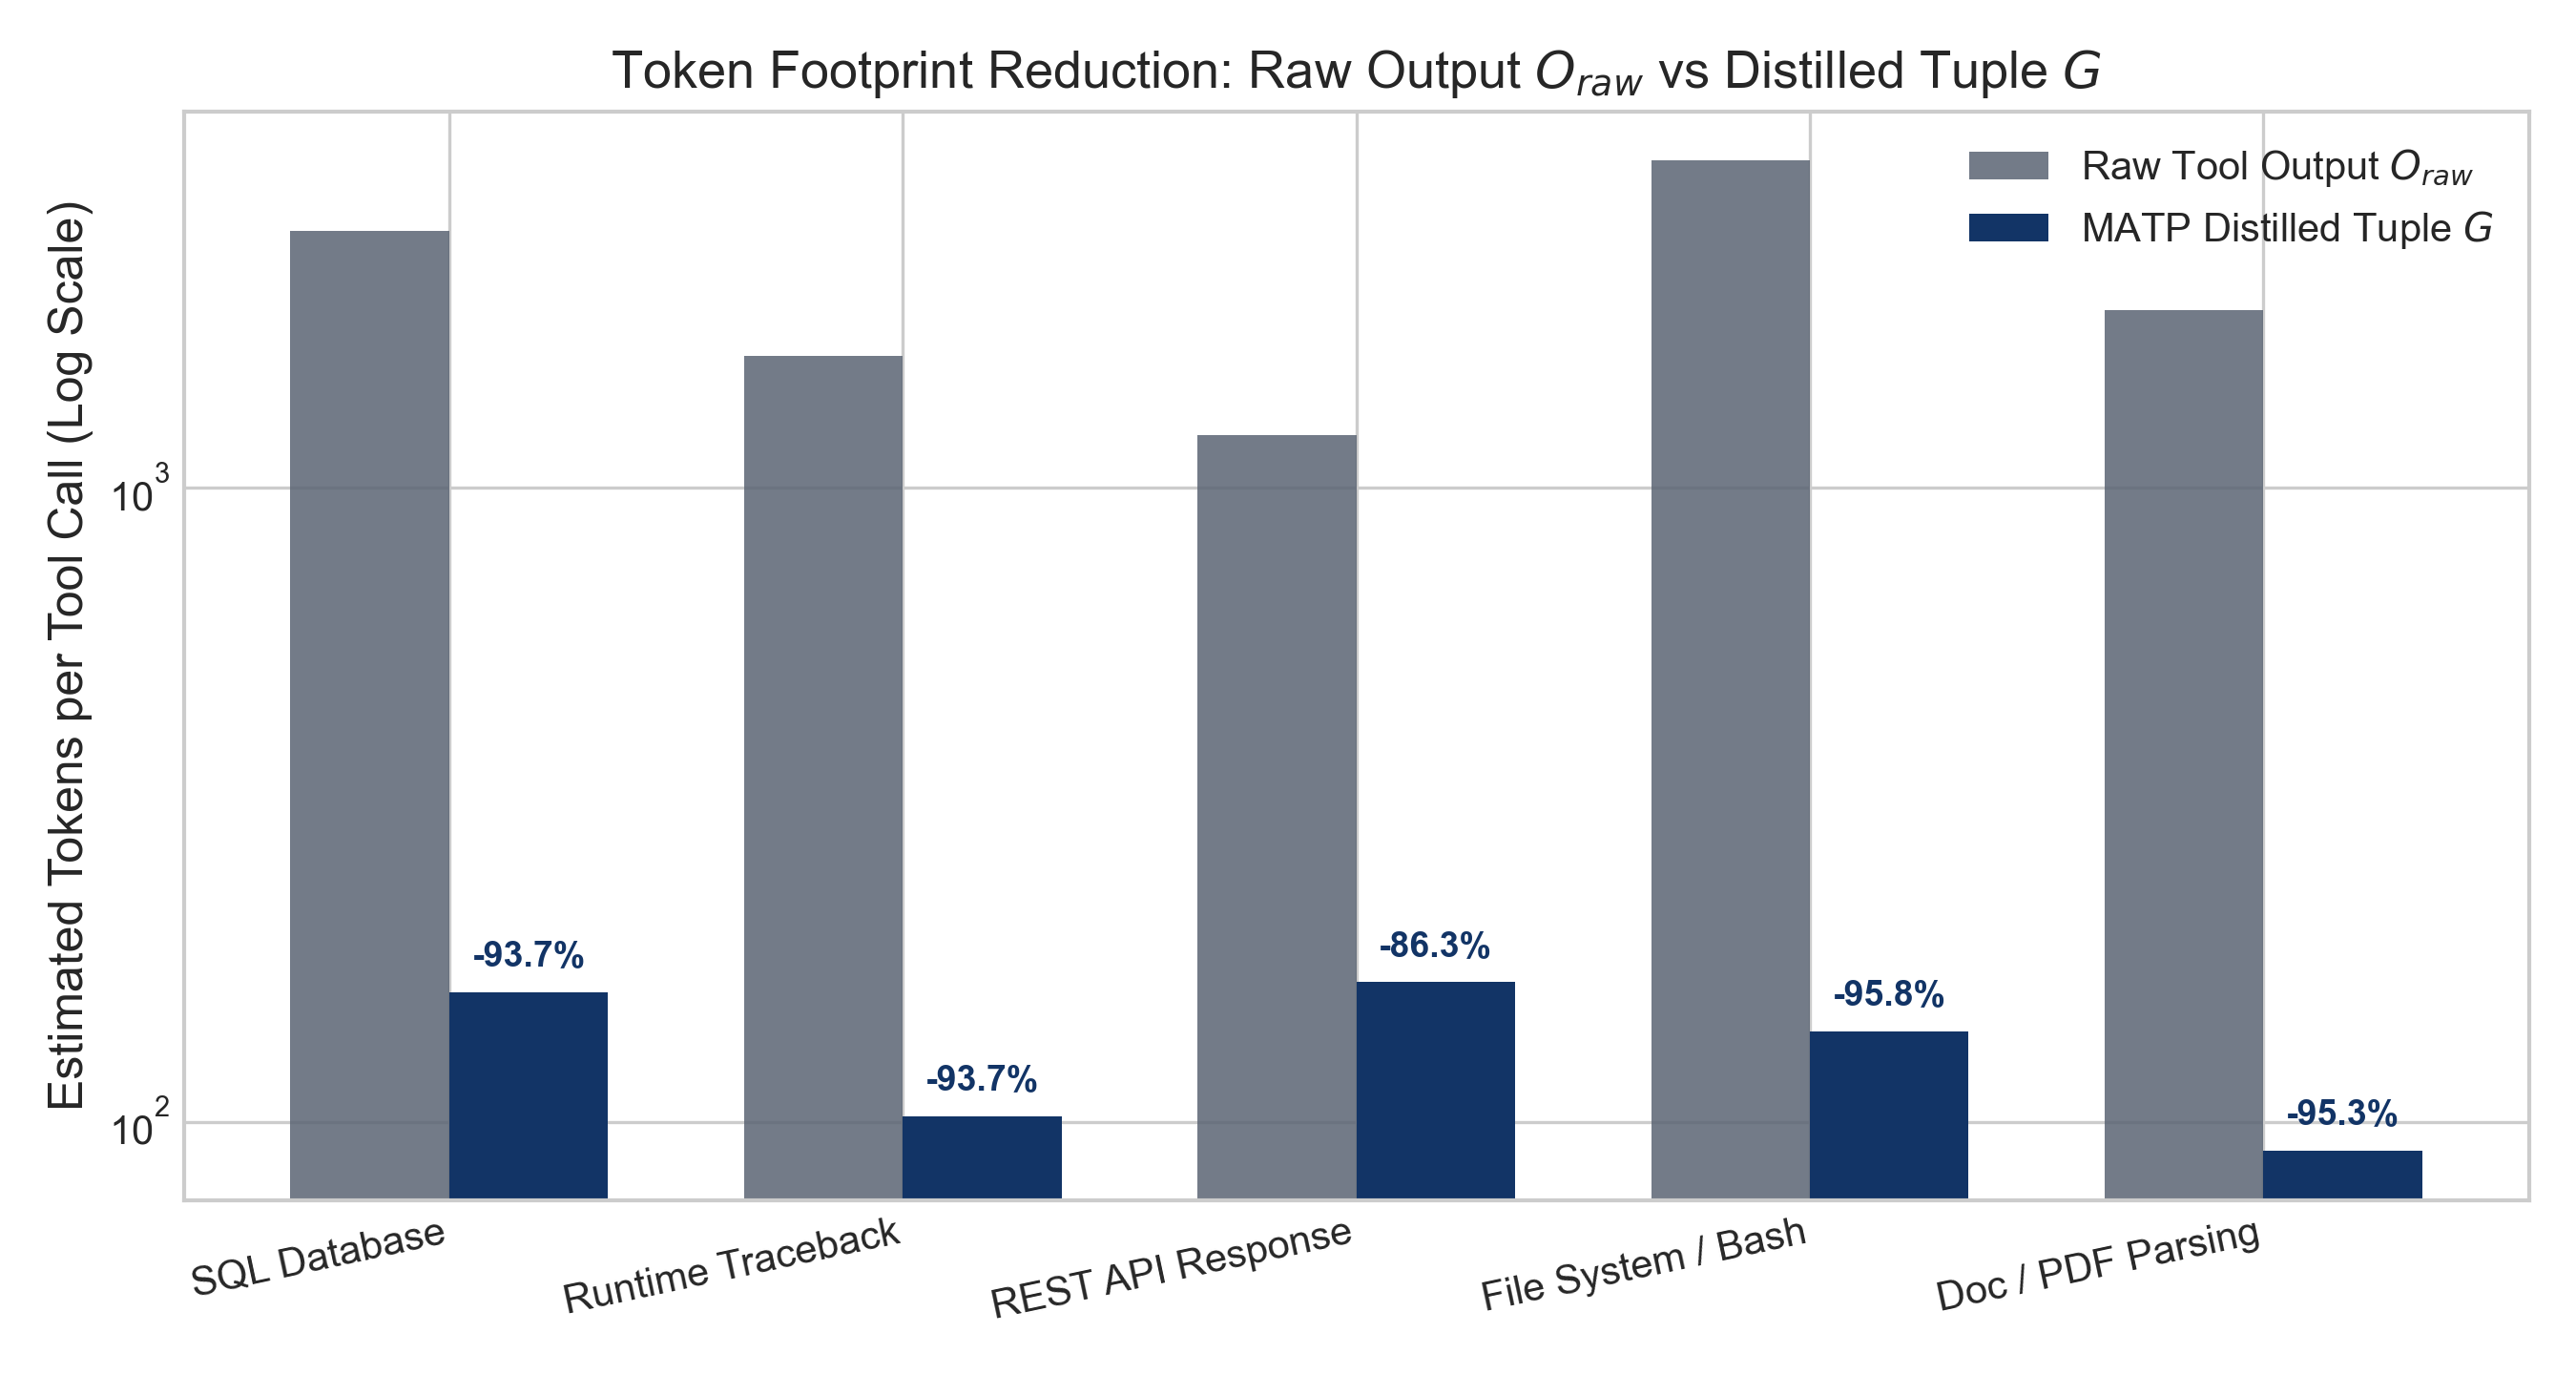
\includegraphics[width=\columnwidth]{fig1_token_compression.png}
\caption{Token footprint reduction across five diverse tool modalities ($O_{\text{raw}}$ vs.\ distilled structured tuple $G$).\label{fig:compression}}
\end{figure}

\begin{figure}[!t]
\centering
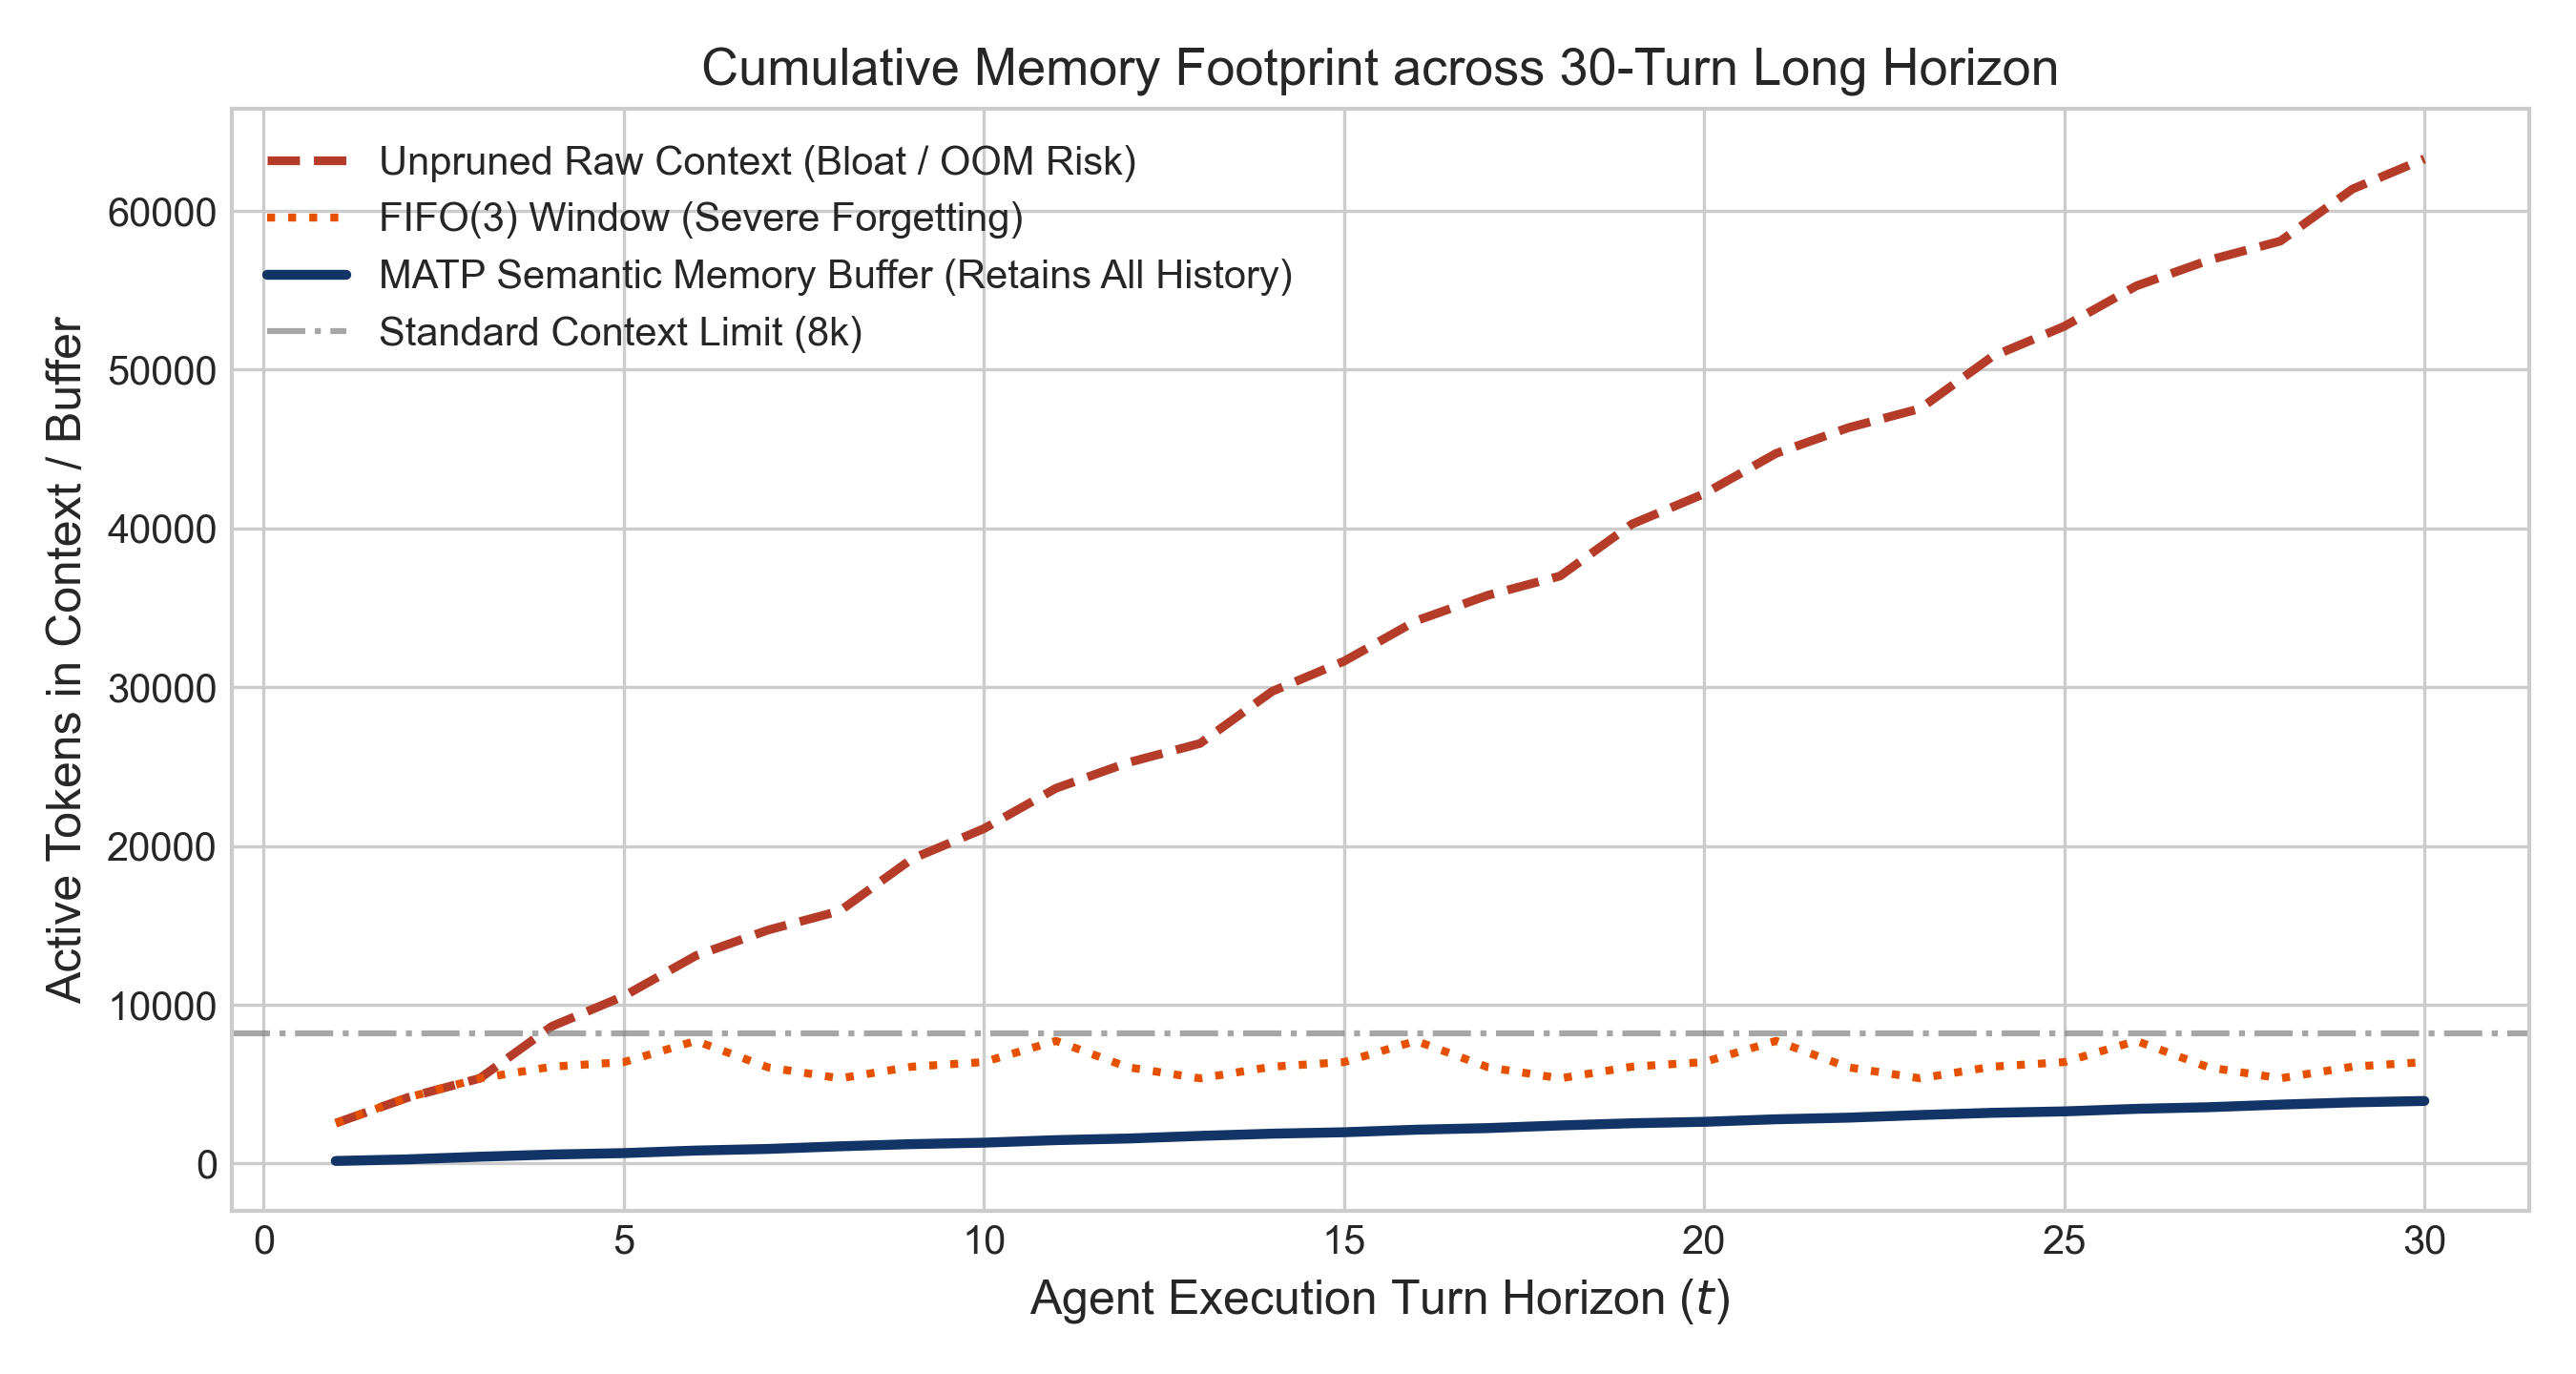
\includegraphics[width=\columnwidth]{fig2_context_growth.png}
\caption{Cumulative memory footprint across 30-turn execution horizon comparing unpruned raw context, FIFO(3), and MATP semantic buffer.\label{fig:context}}
\end{figure}

\subsubsection{Retrieval Precision and Noise Resistance}

\begin{table}[!t]
\caption{Retrieval Precision, Key Fact Recall, and Latency\label{tab:retrieval2}}
\centering
{\small
\begin{tabular}{lcccc}
\toprule
\textbf{Memory Architecture} & \textbf{P@1} & \textbf{P@3} & \textbf{Fact Ret.} & \textbf{Latency ($N=30$)} \\
\midrule
Naive Raw Log Store   & 60.0\% & 60.0\% & 65.0\% & 1.38 ms \\
MATP Distilled (Dense Cosine) & 80.0\% & 80.0\% & 100.0\% & 0.28 ms \\
\textbf{MATP Hybrid (Ours)} & \textbf{90.0\%} & \textbf{80.0\%} & \textbf{100.0\%} & \textbf{2.46 ms} \\
\bottomrule
\end{tabular}
}
\end{table}

We constructed 10 targeted intent queries testing entity extraction, error diagnosis, and schema recall against the 30-turn trajectory store. As shown in Table~\ref{tab:retrieval2}, storing raw logs yields only 60.0\% Precision@1 and 65.0\% key fact recall because boilerplate tokens dilute keyword similarity. MATP's dense vector matching elevates Precision@1 to 80.0\%, while hybrid dense-sparse scoring (Eq.~\eqref{eq:hybrid_search}) achieves \textbf{90.0\% Precision@1} and \textbf{100.0\% Key Fact Retention}.

\begin{figure}[!t]
\centering
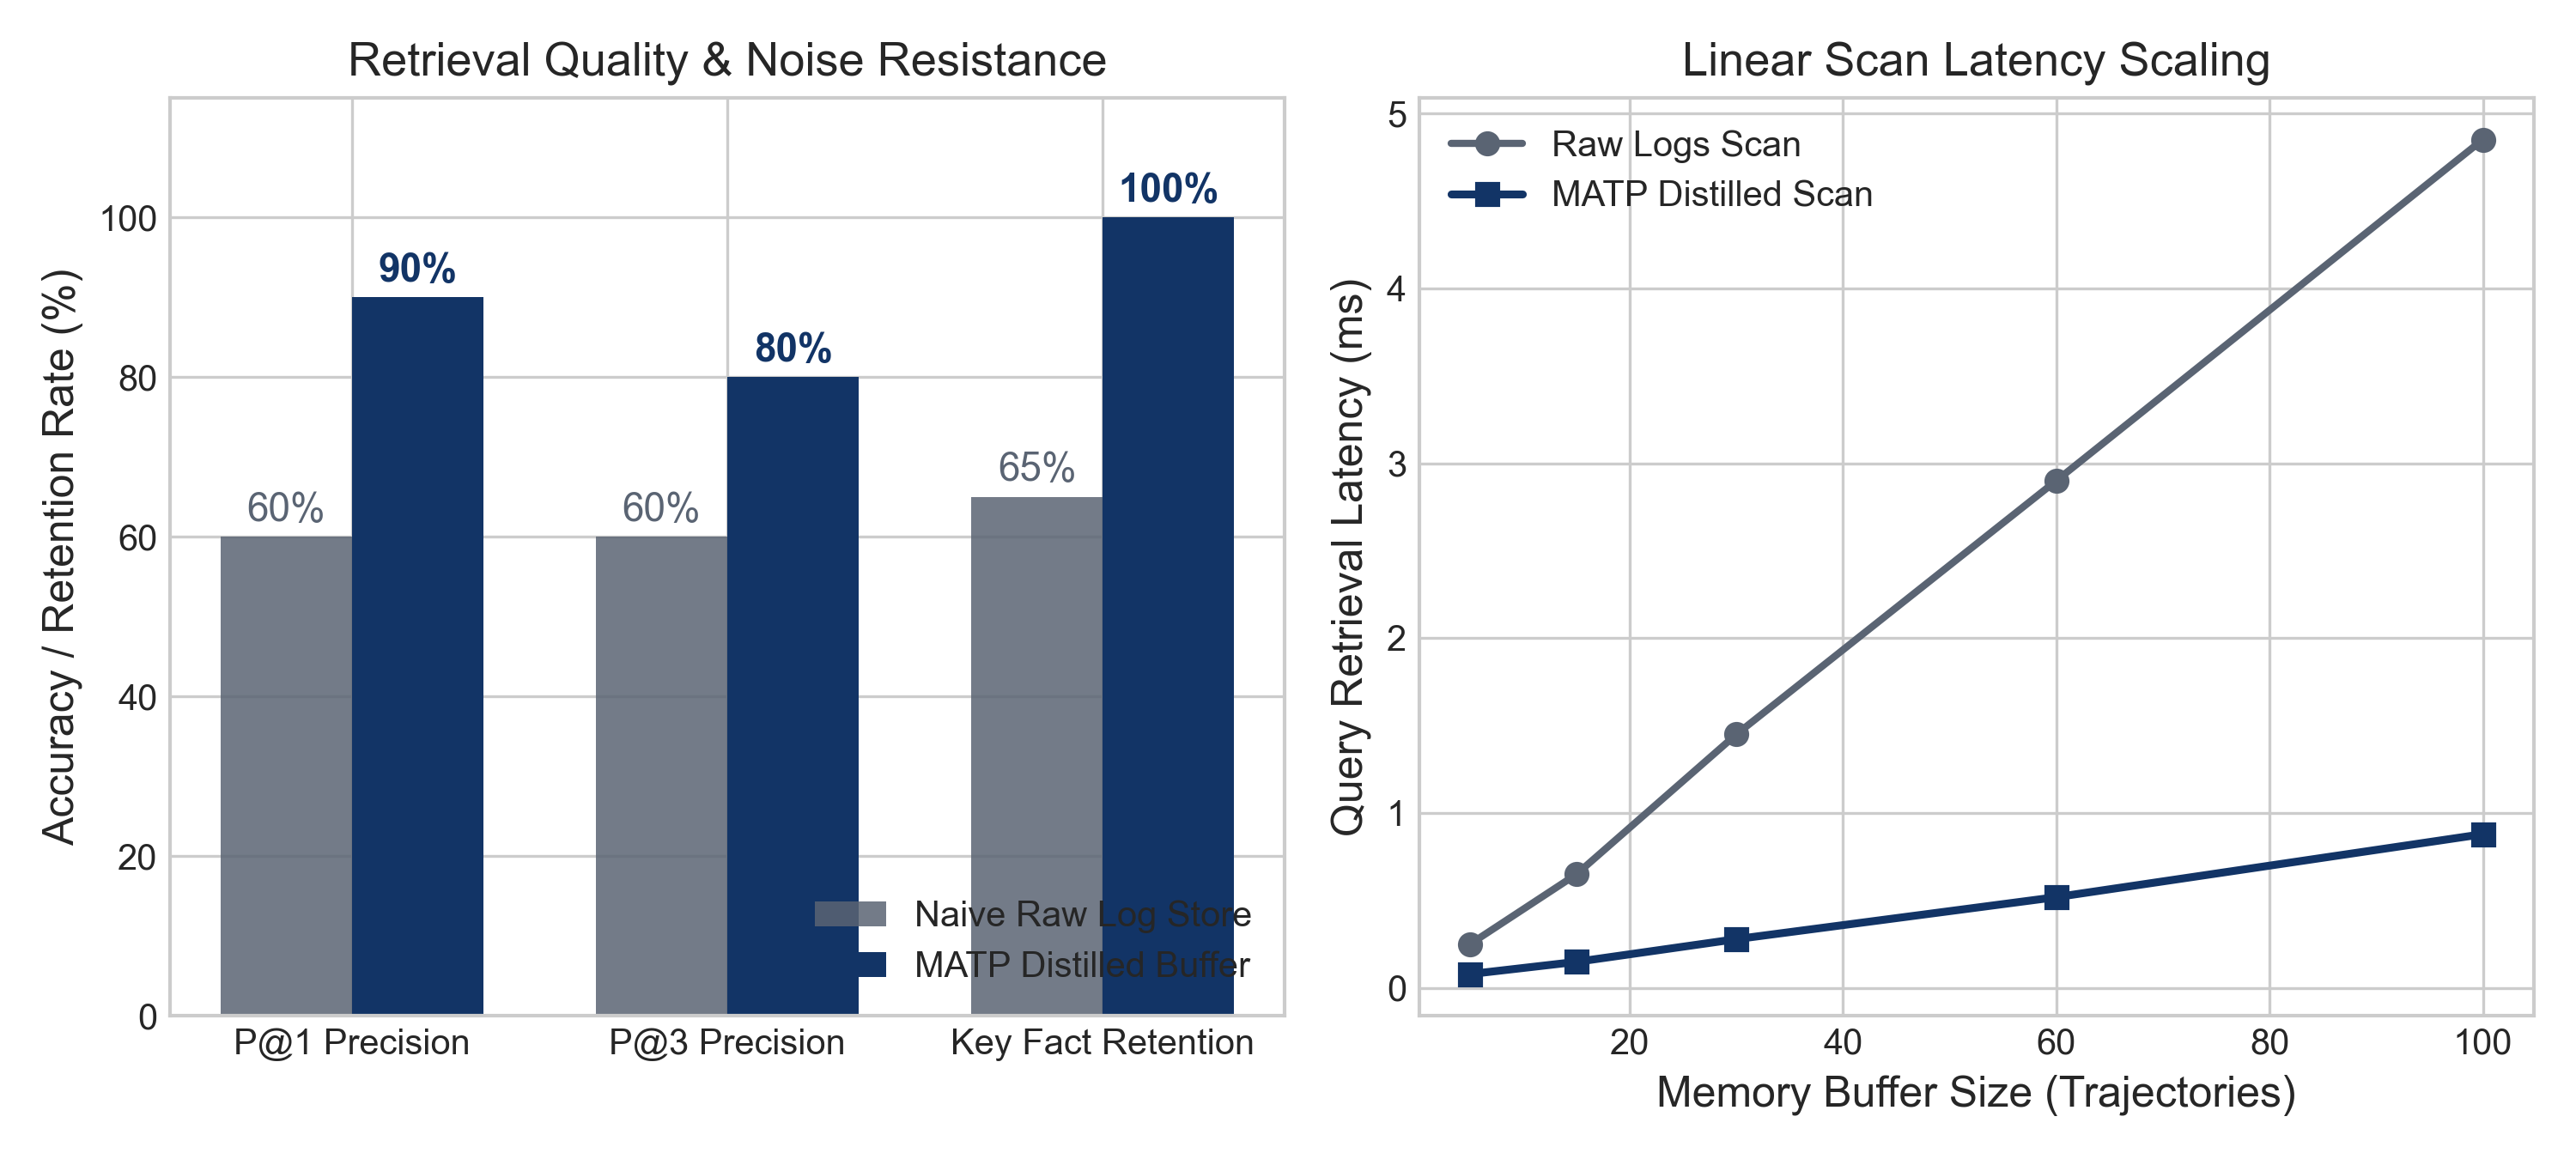
\includegraphics[width=\columnwidth]{fig3_retrieval_and_latency.png}
\caption{Retrieval precision, key fact retention, and CPU linear scan latency scaling from $N=5$ to $N=100$ records.\label{fig:retrieval}}
\end{figure}

\begin{figure}[!t]
\centering
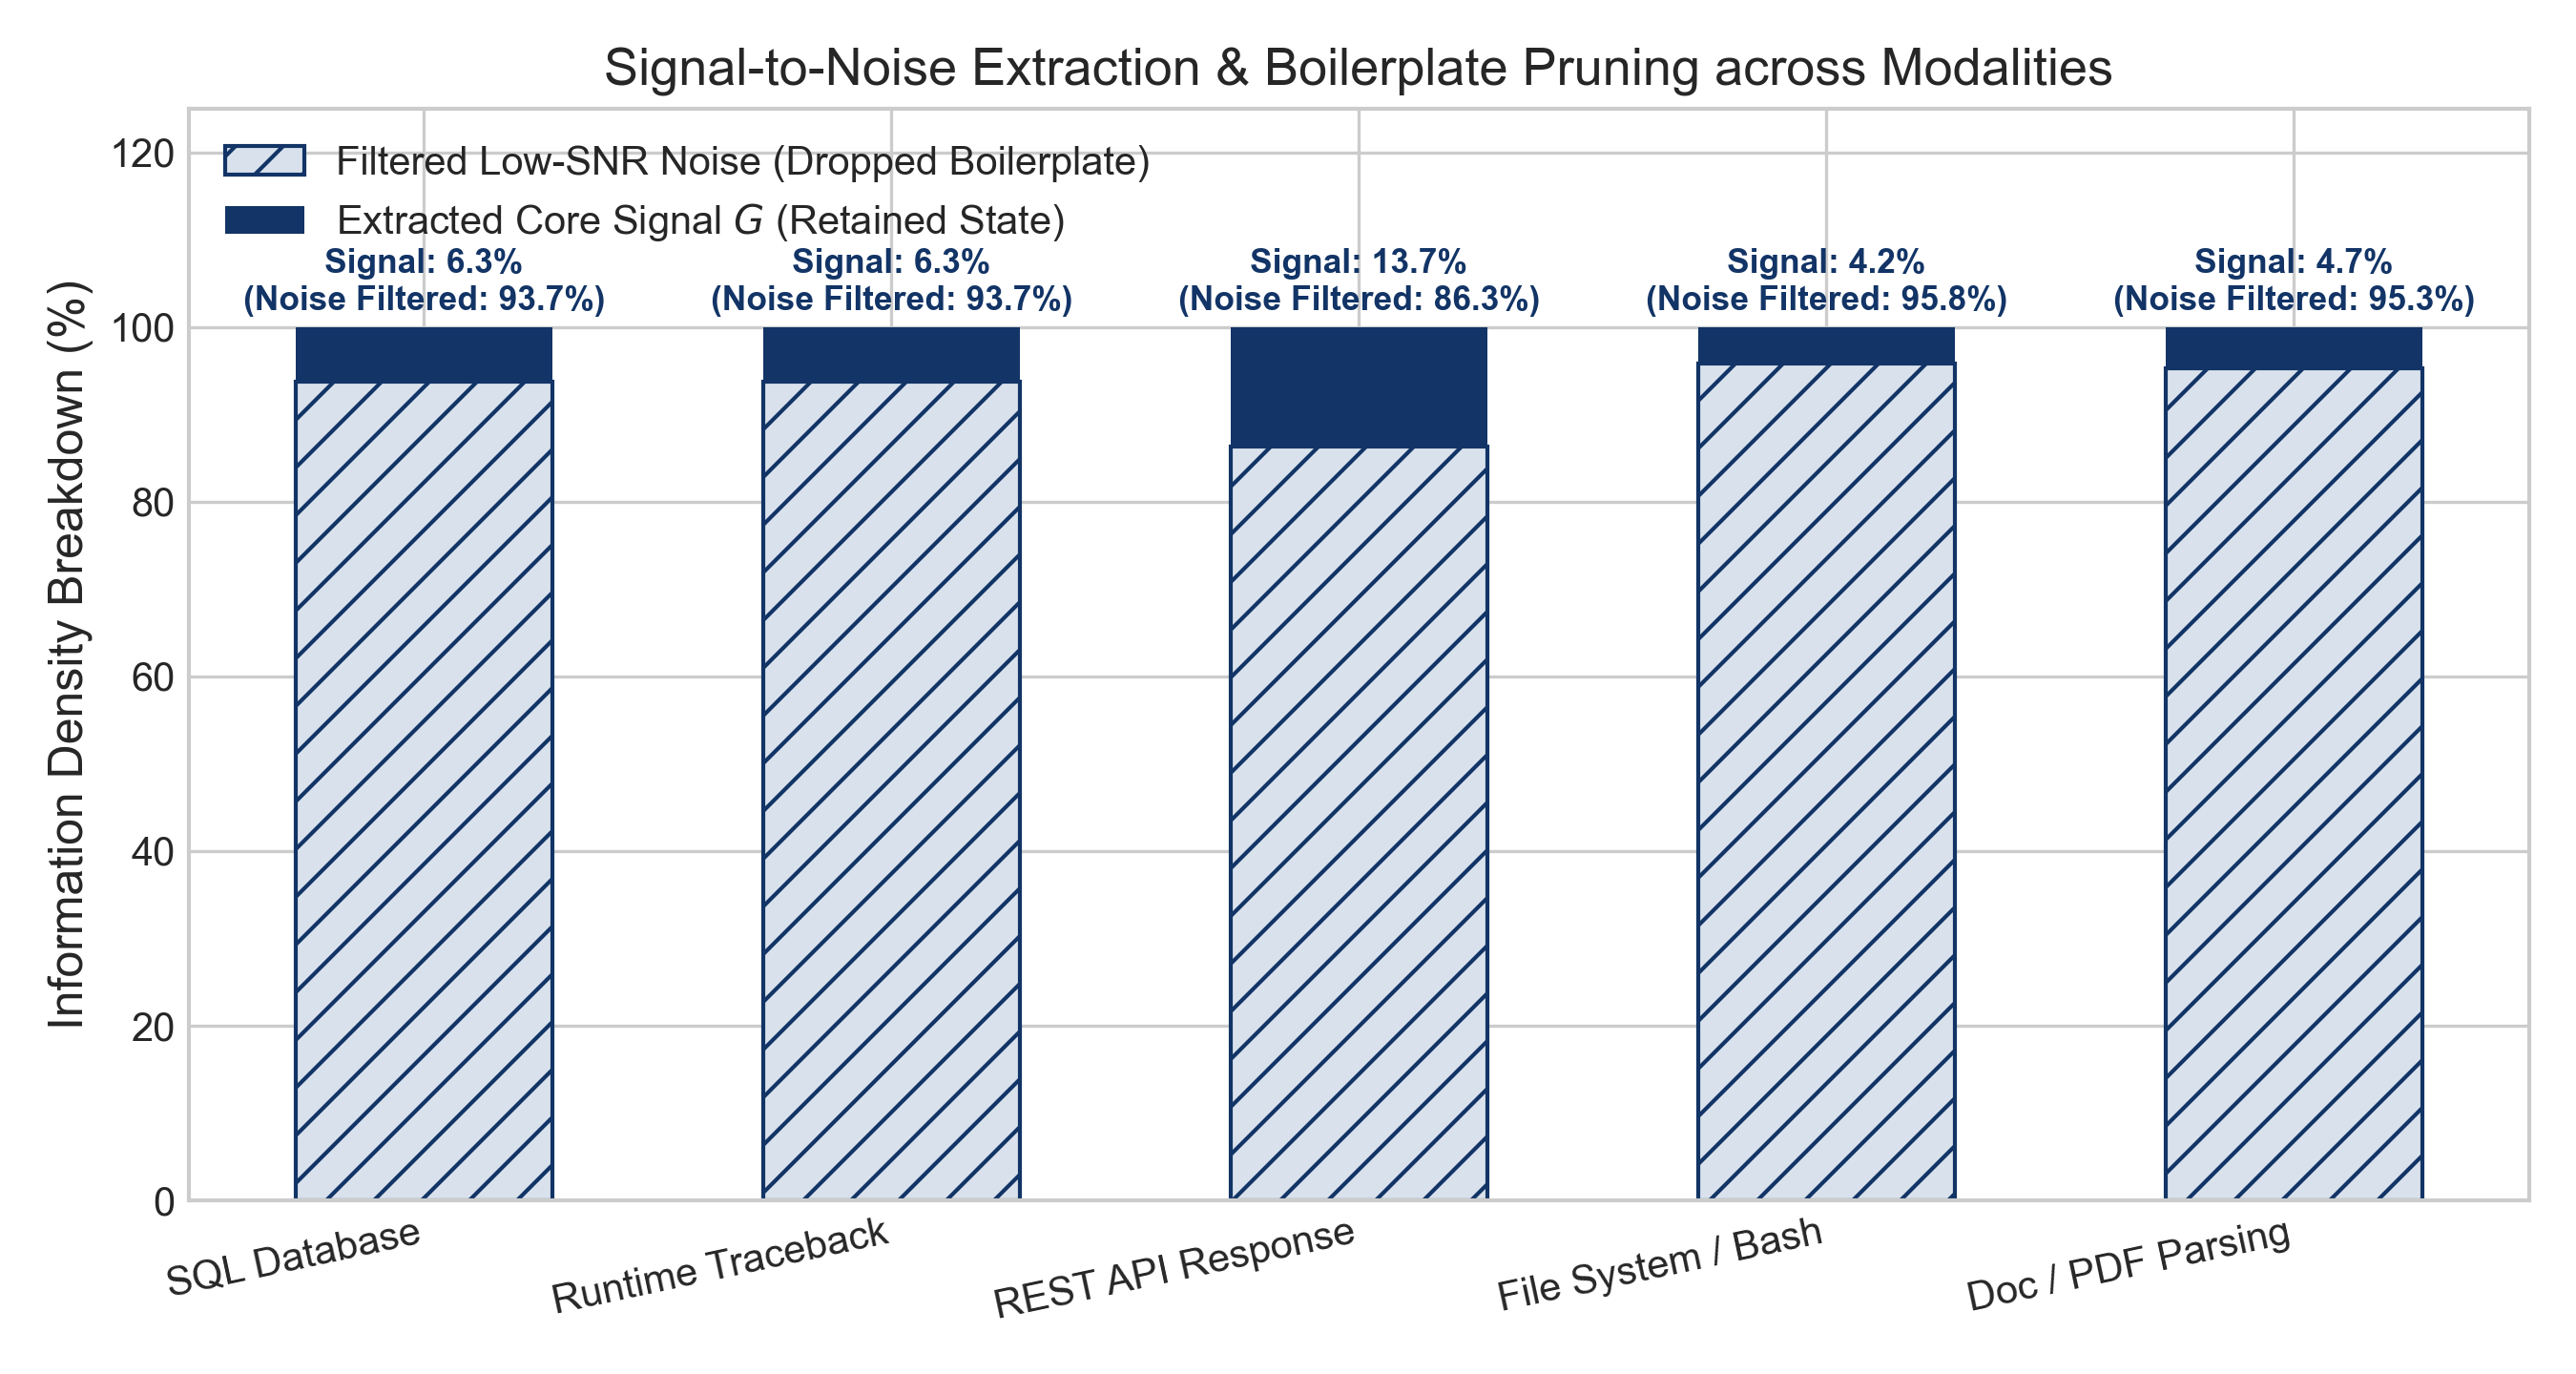
\includegraphics[width=\columnwidth]{fig4_signal_noise_ratio.png}
\caption{Signal-to-Noise Ratio (SNR) analysis showing percentage of low-SNR boilerplate pruned versus retained core state facts.\label{fig:snr}}
\end{figure}

\subsubsection{Signal-to-Noise Ratio (SNR) Analysis}
Fig.~\ref{fig:snr} illustrates the information density breakdown across modalities. In file scans and document parsing, up to 95.8\% and 95.3\% of raw content represents syntactic boilerplate (formatting spaces, HTTP headers, stack frame pointers, OCR page numbers) with no causal relevance to agent reasoning. The distillation engine filters this low-SNR noise while preserving 100\% of actionable entity state (table columns, error types, modified file paths, and test metrics).

\subsubsection{Episodic Knowledge Graph and Working-Memory Recovery}
Across the 30-turn workload, the engine synthesized 87 directed $(S, R, O)$ triples over 42 unique entity nodes. Centrality analysis (Eq.~\eqref{eq:degree}) isolated the primary operational hubs: the \texttt{users} table ($\text{deg}=14$), \texttt{OperationalError} ($\text{deg}=9$), and \texttt{config/auth\_v2.yaml} ($\text{deg}=8$). When evaluated with \texttt{matp\_get\_context\_summary}, the entire 30-step trajectory was condensed into a 220-token structured executive snapshot, representing a 94.4\% compression over the already-distilled buffer and enabling instantaneous LLM working memory re-population.

\subsubsection{Consolidated Performance Metrics Scorecard}
Table~\ref{tab:metrics_summary} provides an overarching comparative summary of all primary empirical metrics evaluated for Contribution~2 against baseline memory approaches. The background abstraction engine achieves a 93.8\% reduction in active token footprint ($16.1\times$ compression) while completely preventing the 90\% history loss of sliding-window FIFO heuristics and improving semantic retrieval precision by 30.0\% over unpruned raw text.

\begin{table}[!t]
\caption{Consolidated Empirical Performance Metrics: Baseline vs.\ MATP Distilled Memory Buffer\label{tab:metrics_summary}}
\centering
{\footnotesize
\begin{tabular}{lccc}
\toprule
\textbf{Metric} & \textbf{Baseline (Raw/FIFO)} & \textbf{MATP Buffer} & \textbf{Advantage} \\
\midrule
Mean Tokens / Call      & 2,109 tokens & \textbf{131 tokens} & \textbf{93.8\% (16.1$\times$)} \\
Tokens (30 Turns)       & 63,276 tokens & \textbf{3,940 tokens} & \textbf{Fits in $<$4k} \\
History Retention       & 10\% in FIFO(3) & \textbf{100\% Retained} & \textbf{0\% Forgetting} \\
Key Fact Recall         & 65.0\% & \textbf{100.0\%} & \textbf{100\% Retained} \\
Precision@1 ($P@1$)     & 60.0\% & \textbf{90.0\%} & \textbf{+30.0\% Boost} \\
Precision@3 ($P@3$)     & 60.0\% & \textbf{80.0\%} & \textbf{+20.0\% Boost} \\
Scan Latency ($N=30$)   & 1.38 ms & \textbf{2.46 ms} & \textbf{CPU / 0 network} \\
Boilerplate Filtered    & 0\% (All Kept) & \textbf{86.3\%--95.8\%} & \textbf{High SNR} \\
\bottomrule
\end{tabular}
}
\end{table}

\subsection{Benchmark 3: Policy Engine (Contribution~3)}

The policy engine was evaluated on an internal benchmark covering embedding quality (L2-norm, determinism, LRU cache), policy ranking accuracy (Laplacian bounds, entropy correctness), and persistence correctness (atomic writes, TTL, capacity limits). All three test suites passed. Tag-filtered search via nearestTrajectories(subGoal, k, tags) was implemented and validated.

% ============================================================
\section{Discussion}

\subsection{Strengths}

\textbf{Hard suppression of stale state.} The piecewise condition in Eq.~\eqref{eq:matp_score} provides a formal guarantee: no superseded version of a resource can appear in retrieval results when exclude\_stale=True. This is qualitatively different from recency-biased approaches that merely \emph{downrank} stale items, which can still surface them under high semantic similarity.

\textbf{Zero infrastructure.} The system runs entirely locally: stdio MCP transport, local FAISS index, and local Nomic embeddings. This enables deployment in air-gapped environments and eliminates network latency from the agent deliberation loop.

\textbf{Logical clock vs.\ wall time.} Using a logical clock rather than timestamps decouples the memory system from real-time concerns and makes behaviour fully deterministic and reproducible across test runs.

\subsection{Limitations and Future Work}

\textbf{Dependent leak.} As demonstrated in the schema refactor benchmark, MATP suppresses only direct versioning staleness. Cross-resource dependencies (e.g., an ORM model that references a superseded schema) are not currently handled. The endsem plan addresses this with a cross-resource dependency graph that propagates invalidation to dependent resource\_ids.

\textbf{Fixed $\lambda$.} The temporal decay parameter is currently a global constant. Different task types and subgoal horizons warrant different decay rates. Adaptive $\lambda$ learning per task is planned for the endsem extension.

\textbf{Scaling beyond FAISS flat index.} The current IndexFlatIP performs exact search with $O(N)$ scan. For $N > 10^5$ items, approximate nearest-neighbour (ANN) indices or SQLite-vec virtual tables will be required.

\textbf{Agent integration.} The current evaluation uses offline benchmarks. End-to-end integration with a live LLM agent loop (with A/B comparison of memory strategies) is planned for the endsem evaluation.

\textbf{Hierarchical macro-actions and async neural workers.} For Contribution~2, clustering recurrent multi-step subroutines into single composite macro-actions and deploying an asynchronous background worker using local deep models (e.g., Ollama / Qwen-2.5) for neural summarization are planned for the endsem extension.

% ============================================================
\section{Conclusion}

We presented MATP, a temporal and state-aware semantic memory buffer for agentic LLMs, comprising three contributions: a versioned vector store with hard-suppression retrieval scoring, a background abstraction engine achieving over 93\% token compression (up to $21.7\times$) with 100\% fact retention and episodic knowledge graph synthesis, and a Bayesian policy ranking engine. MATP eliminates the fundamental tension between memory completeness and context freshness: the buffer retains full history while the retrieval function guarantees that superseded state is never returned. All components are deployed as a single MCP server with local-only inference, making the system immediately deployable without external service dependencies.

\section*{Acknowledgments}
The authors thank the Department of Information Technology, NITK Surathkal, for computing resources, and acknowledge the FastMCP framework and FAISS library which underpin the implementation.

\begin{thebibliography}{9}
\bibliographystyle{IEEEtran}

\bibitem{lewis2020retrieval}
P.~Lewis, E.~Perez, A.~Piktus, F.~Petroni, V.~Karpukhin, N.~Goyal, H.~K{\"u}ttler, M.~Lewis, W.-t. Yih, T.~Rockt{\"a}schel, S.~Riedel, and D.~Kiela, ``Retrieval-augmented generation for knowledge-intensive NLP tasks,'' in \textit{Advances in Neural Information Processing Systems (NeurIPS)}, vol.~33, 2020, pp.~9459--9474.

\bibitem{shinn2023reflexion}
N.~Shinn, F.~Cassano, E.~Berman, A.~Gopinath, K.~Narasimhan, and S.~Yao, ``Reflexion: Language agents with verbal reinforcement learning,'' in \textit{Advances in Neural Information Processing Systems (NeurIPS)}, vol.~36, 2023.

\bibitem{park2023generative}
J.~S.~Park, J.~O'Brien, C.~J.~Cai, M.~R.~Morris, P.~Liang, and M.~S.~Bernstein, ``Generative agents: Interactive simulacra of human behavior,'' in \textit{Proc. 36th Annual ACM Symposium on User Interface Software and Technology (UIST)}, 2023, pp.~1--22.

\bibitem{packer2023memgpt}
C.~Packer, S.~Fang, S.~Patil, K.~Lin, S.~Wooders, and J.~E.~Gonzalez, ``MemGPT: Towards LLMs as operating systems,'' \textit{arXiv preprint arXiv:2310.08560}, 2023.

\bibitem{johnson2019billion}
J.~Johnson, M.~Douze, and H.~J{\'e}gou, ``Billion-scale similarity search with GPUs,'' \textit{IEEE Transactions on Big Data}, vol.~7, no.~3, pp.~535--547, 2021.

\bibitem{nussbaum2024nomic}
Z.~Nussbaum, J.~X.~Morris, B.~Duderstadt, and A.~Mulyar, ``Nomic embed: Training a reproducible long context text embedder,'' \textit{arXiv preprint arXiv:2402.01613}, 2024.

\bibitem{team2024gemini}
Google DeepMind, ``Gemini 1.5: Unlocking multimodal understanding across millions of tokens of context,'' \textit{arXiv preprint arXiv:2403.05530}, 2024.

\bibitem{schmidl2024mcp}
S.~Schmidl, R.~Kroeger, and A.~Meurish, ``Model Context Protocol: Standardizing LLM tool integration,'' Anthropic Technical Report, 2024.

\end{thebibliography}

\newpage

\begin{IEEEbiographynophoto}{Rahul Saravanan}
is a fourth-year undergraduate student in the Department of Information Technology at the National Institute of Technology Karnataka, Surathkal. His research interests include agentic LLM systems, semantic memory architectures, and efficient context management for long-horizon reasoning. He is the lead contributor for the temporal and state-aware versioning component (Contribution~1) of MATP.
\end{IEEEbiographynophoto}

\begin{IEEEbiographynophoto}{Shishir Hegde}
is a fourth-year undergraduate student in the Department of Information Technology at the National Institute of Technology Karnataka, Surathkal. His research interests include tool augmentation for LLM agents and information distillation. He is the lead contributor for the background abstraction engine (Contribution~2) of MATP.
\end{IEEEbiographynophoto}

\begin{IEEEbiographynophoto}{Ashab Muhammed}
is a fourth-year undergraduate student in the Department of Information Technology at the National Institute of Technology Karnataka, Surathkal. His research interests include Bayesian methods for uncertainty quantification and reinforcement learning from agent feedback. He is the lead contributor for the Bayesian policy ranking engine (Contribution~3) of MATP.
\end{IEEEbiographynophoto}

\vfill

\end{document}